\chapter{Revisão de literatura}
\label{cap:revisao}
% --------------------------------------------------------------------------

\section{O ecossistema de nanossatélites e a engenharia de sistemas nacional}
\label{sec:ecossistema}

A consolidação do padrão CubeSat, estruturado originariamente pela \textit{CubeSat Design Specification} (CALIFORNIA POLYTECHNIC STATE UNIVERSITY, 2022), transformou a dinâmica da engenharia espacial ao substituir o desenvolvimento artesanal de satélites por arquiteturas modulares orientadas a interfaces padronizadas. No cenário nacional, a Agência Espacial Brasileira (AEB) estabelece diretrizes rigorosas para o ciclo de vida e a qualificação de nanossatélites acadêmicos e institucionais. Conforme sistematizado na \textit{Apostila da Temática -- Projeto Estrutural} (AEB, 2026), a viabilidade de uma missão de pequeno porte repousa na conciliação harmônica entre os objetivos de carga útil e as restrições impostas pelo veículo lançador. 

Nesse contexto, projetos pioneiros como o nanossatélite universitário ITASAT-1 (CARRARA \textit{et al.}, 2017), desenvolvido pelo Instituto Tecnológico de Aeronáutica (ITA) em cooperação com o Instituto Nacional de Pesquisas Espaciais (INPE), evidenciaram a centralidade das campanhas de Montagem, Integração e Testes (AIT) realizadas no Laboratório de Integração e Testes (LIT/INPE). O chassi estrutural atua como espinha dorsal da plataforma, sendo responsável por suportar os esforços inerciais de lançamento, manter o alinhamento de instrumentos ópticos e dissipar os choques mecânicos decorrentes das operações de separação orbital em baixa órbita terrestre (\textit{Low Earth Orbit} -- LEO).

\section{Dinâmica de lançamento e ejeção}
\label{sec:dinamica-ejecao}

O envelope mecânico a que um nanossatélite é submetido divide-se operacionalmente em duas fases críticas de carregamento: a ascensão propulsiva do veículo lançador e o evento transiente de ejeção orbital. Durante o voo atmosférico e a queima dos estágios propulsores, a estrutura primária do CubeSat comporta-se como um caminho de carga secundário, sujeita à sobreposição de acelerações quase estáticas de manobra, cargas acústicas de alta intensidade e, predominantemente, a um espectro estocástico de vibração aleatória gerado pela combustão dos motores e pela camada limite turbulenta (SAKAY, 2026). Os requisitos normativos do \textit{General Environmental Verification Standard} (GEVS) (NASA, 2013) exigem que a estrutura do nanossatélite possua rigidez suficiente para assegurar desacoplamento dinâmico perante os modos fundamentais do lançador, com frequência própria inicial $f_1 \ge \SI{100.0}{\hertz}$, impedindo a ocorrência de amplificação ressonante catastrófica (MALAVOLTA; MORENO, 2026).

A interface de maior criticidade mecânica direta localiza-se no interior do mecanismo de liberação, historicamente consolidado a partir do desenvolvimento do \textit{Poly-Picosatellite Orbital Deployer} (P-POD) pela California Polytechnic State University (PUIG-SUARI; TURNER; AHLGREN, 2002). O dispensador P-POD, esquematizado na Figura~\ref{fig:ppod}, consiste em um invólucro tubular de alumínio que confina o satélite durante todo o voo de ascensão, protegendo o veículo lançador e as cargas úteis primárias contra qualquer desprendimento acidental. 

\begin{figure}[htb]
  \caption{Diagrama explodido e interfaces mecânicas do dispensador orbital P-POD}
  \label{fig:ppod}
  \begin{center}
    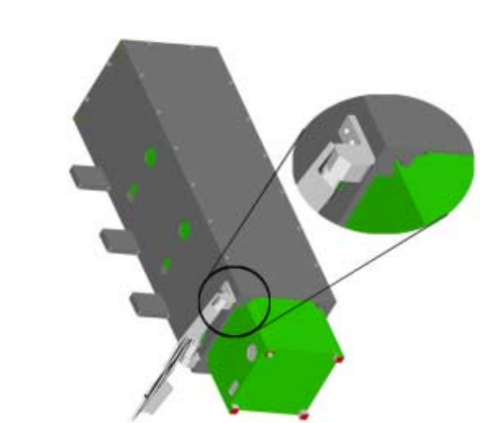
\includegraphics[width=0.7\textwidth]{figuras/ppod_explodido.png}
  \end{center}
  \fonte{Adaptado de Puig-Suari, Turner e Ahlgren (2002).}
\end{figure}

Do ponto de vista cinemático e tribológico, o confinamento no P-POD impõe que os quatro cantos longitudinais do CubeSat atuem como trilhos-guia deslizantes no interior das canaletas tubulares. Na montagem de voo e em ensaios de qualificação em mesas vibratórias acopladas a casulos de ensaio (\textit{Test POD}), os trilhos não são engastados, mas sim restringidos por contato mecânico unilateral sujeito a uma folga diametral nominal (\textit{clearance} de \SIrange{0.1}{0.3}{\milli\metre}), apoiando-se axialmente na interface inferior de sapatas e pinos de encosto da base ($Z = 0$). Durante os ensaios de vibração estocástica e transientes de lançamento, essa folga construtiva induz fenômenos de descolamento periódico, impacto intermitente e vibração com folga (\textit{chattering}), os quais alteram a resposta dinâmica linear do sistema e reduzem a primeira frequência natural aparente em relação a condições idealizadas de engastamento perfeito. Restrições estritas de tolerância dimensional e a necessidade de prevenir o travamento mecânico (\textit{jamming}) ou a microssoldagem a frio sob alto vácuo exigem que esses trilhos tenham seção sólida de \rail{}, cantos arredondados ($R \ge \SI{1.0}{\milli\metre}$) e acabamento superficial com anodização dura tipo III (PTFE impregnado) com rugosidade $Ra \le \SI{1.6}{\micro\metre}$ (PUIG-SUARI \textit{et al.}, 2002). Consequentemente, torna-se geometricamente mandatório que os trilhos do nanossatélite permaneçam maciços e contínuos, de modo que a otimização de alívio de massa e atenuação vibratória seja direcionada exclusivamente aos painéis internos do chassi.

O evento de ejeção é deflagrado pela liberação da porta frontal do dispensador, descarregando a energia potencial elástica acumulada na mola helicoidal principal sobre a placa empurradora (\textit{pusher plate}). A dinâmica translacional de ejeção do satélite ao longo do curso de ejeção é governada pela equação de movimento expressa na Equação~\eqref{eq:ejecao} (LIMA; MANEA; SANTOS, 2021):
\begin{equation}
  M\,\ddot{z} + \mu N \operatorname{sgn}(\dot{z}) = P_0 - c\,z
  \label{eq:ejecao}
\end{equation}
em que $M$ denota a massa combinada do CubeSat e da plataforma empurradora, $\ddot{z}$ representa a aceleração axial instantânea, $P_0$ é a pré-carga inicial da mola comprimida, $c$ é a constante de rigidez da mola, $\mu$ é o coeficiente de atrito cinemático contra as guias do tubo, $N$ é a força normal de contato induzida por desalinhamentos e $z$ corresponde ao deslocamento axial percorrido até o curso total ($z = z_{\text{curso}}$). 

Ao término do curso de impulsão, a placa empurradora desacelera bruscamente ao colidir contra o batente mecânico final do dispensador, transferindo um pulso transiente de choque impulsivo de curta duração ($\Delta t \sim \SIrange{1}{3}{\milli\second}$) que se propaga pelos trilhos do nanossatélite no instante de sua liberação em órbita livre (LIMA \textit{et al.}, 2021). A severidade desse evento dinâmico é quantificada pelo Espectro de Resposta ao Choque (\textit{Shock Response Spectrum} -- SRS, com fator de qualidade $\mathcal{Q} = 10$), impondo acelerações de pico que podem superar \SI{500}{\gacc} em frequências superiores a \SI{1000}{\hertz}.

Adicionalmente, esse impulso inicial excita a dinâmica de múltiplos corpos acoplados do satélite. Em plataformas providas de apêndices flexíveis articulados, como hastes de magnetômetros (\textit{booms}), antenas de comunicação e painéis solares dobráveis, o choque de ejeção pode excitar frequências modais ressonantes dos mecanismos periféricos (MANTOVANI; SANTOS; CARDOSO-RIBEIRO, 2020). Essa interação dinâmica reforça a exigência de que os painéis do chassi primário possuam capacidade passiva intrínseca de filtragem mecânica e atenuação de ondas elásticas, evitando a propagação de transientes de alta frequência que possam danificar as articulações dos apêndices ou descalibrar componentes ópticos.

\section{Metamateriais auxéticos e estruturas híbridas de alto desempenho}
\label{sec:auxeticos}

Para superar a baixa dissipação de energia dos materiais monolíticos contínuos, a engenharia de estruturas tem incorporado metamateriais celulares com coeficiente de Poisson negativo ($\nu < 0$), denominados auxéticos. A caracterização empírica de colmeias metálicas reentrantes bidimensionais manufaturadas por fusão seletiva a laser (SLM) em ligas de alumínio foi investigada por Alomarah \textit{et al.} (2017). Esses autores demonstraram que a resposta mecânica e a magnitude do coeficiente de Poisson negativo dessas matrizes exibem acentuada anisotropia direcional: espécimes solicitados na direção X apresentam rigidez e limites de escoamento consideravelmente inferiores aos observados na direção Y. Corroborando essa dependência direcional no contexto da manufatura aditiva metálica, Ermurat e Da\u{g} (2025) avaliaram a influência combinada da orientação de construção (\textit{build orientation}) e do sentido de aplicação de carga sobre o comportamento compressivo de estruturas auxéticas reentrantes manufaturadas aditivamente. As investigações evidenciaram que o arranjo das camadas depositadas afeta substancialmente os modos de deformação plástica, a capacidade de absorção energética e a suscetibilidade a concentrações locais de tensão nos vértices nodais.

Além da anisotropia elástica e da dependência em relação à orientação de fabricação, matrizes reentrantes convencionais fabricadas por manufatura aditiva sem pós-processamento térmico sofrem de limitações severas de ductilidade. Como verificado experimentalmente por Alomarah \textit{et al.} (2017), a concentração de deformações plásticas nas quinas internas das costelas oblíquas induz a formação prematura de trincas e fratura frágil sob carregamentos quase estáticos, inibindo o desenvolvimento de um platô plástico estendido de absorção energética. A Figura~\ref{fig:falha-reentrante} ilustra os modos típicos de colapso e a propagação de trincas nas junções de células reentrantes 2D sob tração uniaxial.

\begin{figure}[htb]
  \caption{Modos de falha e comportamento cinemático anisotrópico de célula reentrante 2D sob carregamento uniaxial}
  \label{fig:falha-reentrante}
  \begin{center}
    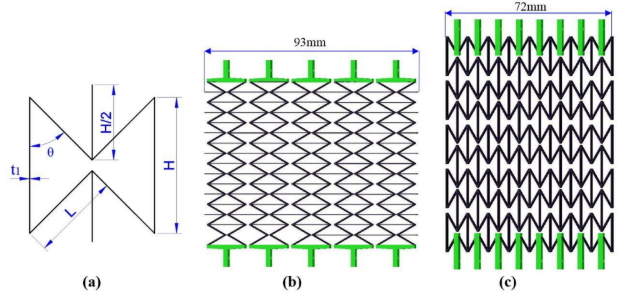
\includegraphics[width=0.85\textwidth]{figuras/modos_falha_reentrante.png}
  \end{center}
  \fonte{Adaptado de Alomarah \textit{et al.} (2017).}
\end{figure}

Para contornar o colapso localizado e estender a capacidade de absorção de choque, geometrias celulares avançadas combinam mecanismos reentrantes com elementos quirais ou bioinspirados. Cui, Zhang e Wang (2025) demonstraram que a incorporação de núcleos quirais rotacionais no interior de colmeias reentrantes, conforme ilustrado na Figura~\ref{fig:hibrida-quiral}, propicia um aumento de até \SI{95}{\percent} na Absorção Específica de Energia (\textit{Specific Energy Absorption} -- SEA) em comparação com topologias puramente reentrantes. 

\begin{figure}[htb]
  \caption{Topologia híbrida de célula celular com elementos quirais internos acoplados a paredes reentrantes}
  \label{fig:hibrida-quiral}
  \begin{center}
    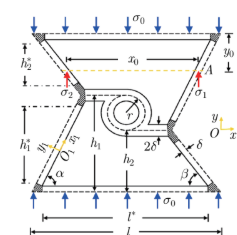
\includegraphics[width=0.55\textwidth]{figuras/celula_hibrida_quiral.png}
  \end{center}
  \fonte{Adaptado de Cui, Zhang e Wang (2025).}
\end{figure}

Apesar do incremento expressivo de absorção de energia propiciado pelas células híbridas quirais reportadas por Cui, Zhang e Wang (2025), tais geometrias impõem severos desafios de fabricabilidade no processo de fusão em leito de pó a laser (L-PBF). A geometria dos nós circulares e ligamentos curvos rotacionais resulta frequentemente em superfícies suspensas com ângulos de inclinação (\textit{overhang}) críticos inferiores a \SI{35}{\degree}, exigindo suportes sacrificiais internos que se tornam inacessíveis para remoção mecânica após a consolidação a laser. Em adição, a complexidade dos canais internos confinados dificulta a evacuação e a recuperação do pó metálico não fundido. Em contrapartida, a célula unitária tridimensional reentrante (3D \textit{re-entrant}) selecionada no presente estudo assegura plena conformidade com as diretrizes de \textit{Design for Additive Manufacturing} (DfAM): a parametrização das costelas garante ângulos de sobressalto $\theta_{\text{overhang}} \ge \SI{35}{\degree}$ ao longo da direção de construção vertical, dispensando integralmente suportes internos sacrificiais e mantendo canais desobstruídos e contínuos para drenagem e despoeiramento em L-PBF.

Sob o ponto de vista da elastodinâmica, tais arranjos arquitetados atuam de maneira análoga a cristais fonônicos, exibindo zonas de atenuação espectral (\textit{phononic bandgaps}) que impedem a transmissão de ondas elásticas em faixas específicas de frequência (LI \textit{et al.}, 2026; FARSHBAF \textit{et al.}, 2025). Essa propriedade física viabiliza o isolamento mecânico passivo de cargas úteis de alta sensibilidade, dispensando o uso de amortecedores elastoméricos adicionais que poderiam degradar por desgaseificação (\textit{outgassing}) no ambiente espacial.

\section{\textit{Design for Additive Manufacturing} (DfAM) e modelos de escala}
\label{sec:dfam}

A viabilização prática de componentes espaciais celulares é intrinsecamente governada pelo paradigma de \textit{Design for Additive Manufacturing} (DfAM). Conforme destacado na revisão de Khan e Riccio (2024), processos de Manufatura Aditiva por Fusão em Leito de Pó a Laser (\textit{Laser Powder Bed Fusion} -- L-PBF) proporcionam liberdade geométrica para a confecção de Estruturas de Densidade Graduada (\textit{Functionally Graded Lattices} -- FGL). A modulação espacial contínua da espessura das costelas e da porosidade celular viabiliza a concentração de rigidez onde os fluxos de tensão são mais intensos, aliviando massa em regiões subutilizadas.

Para estimar a rigidez macroscópica de meios celulares sem recorrer a simulações de malha contínua refinada em cada iteração de projeto, utilizam-se classicamente as leis fenomenológicas de escala propostas por Gibson e Ashby (1997). A relação analítica fundamental correlaciona o módulo de elasticidade efetivo homogeneizado ($E^{*}$) com a densidade relativa da estrutura ($\rho^{*}/\rho_s$) por uma lei de potência:
\begin{equation}
  \frac{E^{*}}{E_s} = C \left( \frac{\rho^{*}}{\rho_s} \right)^{n}
  \label{eq:gibson}
\end{equation}
na qual $E_s$ e $\rho_s$ representam o módulo de Young e a massa específica do material metálico sólido de base, e $C$ e $n$ são constantes empíricas dependentes da topologia celular. Para arquiteturas celulares cujo modo predominante de deformação sob carga elástica é a flexão das costelas oblíquas — caso das células reentrantes —, adota-se classicamente $n \approx 2$ (ZHONG \textit{et al.}, 2023).

Todavia, investigações recentes apontam desvios significativos do modelo clássico de Gibson-Ashby em componentes manufaturados por L-PBF. Zhong \textit{et al.} (2023) salientam que a Equação~\eqref{eq:gibson} assume a hipótese de vigas esbeltas de Euler-Bernoulli, válida apenas para baixas densidades relativas ($\rho^{*}/\rho_s < \num{0.3}$) e razões comprimento-diâmetro de haste $L/D > 5$. Em contrapartida, estruturas otimizadas para satélites operam frequentemente com densidades relativas moderadas e elevadas ($\rho^{*}/\rho_s \ge \num{0.35}$), regime no qual os esforços axiais e o cisalhamento transversal tornam-se preponderantes.

Conforme demonstrado por Zimmerman \textit{et al.} (2026), o modelo clássico de potência perde precisão analítica no limite do sólido maciço ($\rho^{*}/\rho_s \to 1$), uma vez que não prevê a transição assintótica da resposta governada pela cinemática celular para o comportamento constitutivo do material contínuo. Além disso, irregularidades geométricas microestruturais inerentes ao L-PBF — tais como rugosidade superficial em superfícies inclinadas, aderência de partículas de pó semidilatadas e variações locais no diâmetro do feixe de laser — degradam a rigidez efetiva em comparação com geometrias computacionais ideais (ZIMMERMAN \textit{et al.}, 2026).

Para incorporar esses efeitos e restabelecer a precisão analítica em meios celulares graduados, Beigrezaee, Jalali e Pugno (2026) desenvolveram uma formulação corrigida baseada na introdução de parâmetros modificadores:
\begin{equation}
  \frac{E^{*}}{E_s} = \alpha\,\beta\,C \left( \frac{\rho^{*}}{\rho_s} \right)^{n}
  \label{eq:refinado}
\end{equation}
em que $\alpha$ é o coeficiente de correção determinístico para o gradiente de espessura de parede ao longo do volume, e $\beta$ quantifica o fator de degradação elástica oriundo de imperfeições estocásticas e porosidades induzidas pelo processo de fusão aditiva (BEIGREZAEE \textit{et al.}, 2026). A calibração dos fatores $\alpha$ e $\beta$ permite ancorar as previsões do modelo substituto neural em bases fenomenológicas sólidas.

\section{Integridade estrutural e fadiga em estruturas celulares}
\label{sec:fadiga}

A qualificação aeroespacial de um chassi primário em liga de AlSi10Mg fabricado por L-PBF requer a garantia estrita de resistência mecânica contra a fadiga vibracional estocástica imposta pelo veículo lançador (SLEJKO \textit{et al.}, 2023). Em estruturas celulares metálicas, a presença de descontinuidades geométricas e microestruturais — tais como porosidade por aprisionamento de gás, falta de fusão interfacial e rugosidade superficial dispersa — impede o uso de abordagens clássicas baseadas em fatores teóricos de concentração de tensões elásticas ($K_t$) ou tensões nominais médias (COLLINI; MENEGHETTI, 2024).

Para superar essa limitação e estabelecer uma metodologia de dimensionamento tolerante a defeitos (\textit{defect-tolerant design}), adota-se a formulação da Mecânica da Fratura Linear Elástica (LEFM). Conforme demonstrado por Collini e Meneghetti (2024), as junções nodais e reentrâncias das células podem ser modeladas como entalhes geométricos agudos em V com raio de ponta pequeno, sendo o campo de tensões locais descrito pelo Fator de Intensidade de Tensão de Entalhe (\textit{Notch Stress Intensity Factor} -- NSIF) em Modo I:
\begin{equation}
  \Delta K_1^{V} = \sqrt{2\pi}\,\lim_{r \to 0} \left[ \Delta\sigma_{\theta\theta}(r)\; r^{\,1-\lambda_1} \right]
  \label{eq:nsif}
\end{equation}
em que $\Delta K_1^{V}$ representa a amplitude do NSIF em Modo I, $\Delta\sigma_{\theta\theta}$ é a componente de tensão normal circunferencial atuante a uma distância radial $r$ do vértice do entalhe, e $1-\lambda_1$ denota a ordem da singularidade elástica assintótica de Williams, dependente do ângulo de abertura do entalhe nodal.

A integração da abordagem LEFM acoplada ao Método da Tensão de Pico (\textit{Peak Stress Method} -- PSM) em modelos de elementos finitos permite correlacionar o estado de tensão nodal gerado pela vibração aleatória diretamente com o limiar de propagação de trincas por fadiga da liga AlSi10Mg ($\Delta K_{th} = \SI{2.5}{\mega\pascal\sqrt{\metre}}$) (COLLINI; MENEGHETTI, 2024). Assim, o processo de otimização topológica assegura que as tensões estocásticas de pico ($3\sigma$) nos nós da estrutura permaneçam estritamente abaixo do limiar de propagação, garantindo a integridade do componente durante a fase de qualificação de voo.

\section{Modelos substitutos neurais guiados por física e sistemas multiagente na engenharia aeroespacial}
\label{sec:pgnn-agentes}

A determinação das geometrias celulares ótimas por meio de algoritmos evolutivos multiobjetivo, como o NSGA-II (DEB \textit{et al.}, 2002), impõe a execução de dezenas de milhares de avaliações de candidatas. A realização direta desse volume de simulações por Elementos Finitos (FEA) tridimensionais em malhas refinadas de paredes celulares delgadas é computacionalmente impraticável, exigindo horas de processamento para cada solução (ZHENG \textit{et al.}, 2024).

Para contornar esse gargalo, empregam-se Modelos Substitutos (\textit{surrogates}) treinados com aprendizado profundo. Para mitigar o risco de predições fisicamente espúrias ou de extrapolações não monotônicas intrínsecas a modelos empíricos de caixa preta, a metodologia deste trabalho estrutura uma Rede Neural Guiada por Física (\textit{Physics-Guided ResNet}). A função de perda supervisionada composta incorpora penalidades fenomenológicas diretamente durante o treinamento:
\begin{equation}
  \mathcal{L}_{\text{total}} = \mathcal{L}_{\text{MSE}} + \lambda_{\text{phys}}\,\mathcal{L}_{\text{Gibson-Ashby}} + \lambda_{\text{mono}}\,\mathcal{L}_{\text{monotonicidade}}
  \label{eq:perda-conceito}
\end{equation}
em que $\mathcal{L}_{\text{MSE}}$ quantifica o erro quadrático médio em relação ao conjunto de simulações numéricas de alta ordem (Ansys MAPDL), $\mathcal{L}_{\text{Gibson-Ashby}}$ penaliza desvios assintóticos das leis de escala celulares para regimes de baixa densidade, e $\mathcal{L}_{\text{monotonicidade}}$ impõe que acréscimos na espessura de parede das células promovam elevações estritamente monótonas na rigidez efetiva e na primeira frequência própria fundamental ($f_1$).

Para governar a interação entre triagem geométrica, inferência neural e checagem de conformidade normativa, adota-se o paradigma de Grafos de Estados Finitos Determinísticos (\textit{Deterministic StateGraph Workflow}) implementado por meio da biblioteca LangGraph. Ao contrário de arquiteturas de agentes reativos baseados em modelos de linguagem com tomadas de decisão probabilísticas, o pipeline aqui desenvolvido opera como um Grafo Acíclico Dirigido (DAG) estritamente determinístico, fundado sobre contratos de dados imutáveis e fortemente tipados (\code{CubeSatState}). Esse arranjo desacopla o fluxo em nós especialistas com responsabilidade única: o portão de manufaturabilidade aditiva (\code{CadDfamAgent}), o estimador dinâmico neural de submilissegundos (\code{NeuralSurrogateAgent}) e o módulo de qualificação ambiental espacial (\code{GevsQualifierAgent}), coordenados pelo controlador supervisor (\code{OrchestratorAgent}). 

Na engenharia de sistemas espaciais e computação científica de alto desempenho, fluxos determinísticos dessa natureza são tradicionalmente geridos por orquestradores de tarefas como Prefect, Snakemake ou Apache Airflow, os quais se destacam na execução distribuída em clusters HPC e gerenciamento de cache. No presente arcabouço, a seleção do LangGraph fundamenta-se na facilidade de instanciação de máquinas de estados tipadas em Python puro, com suporte nativo a bifurcações condicionais (\textit{fail-fast routing}), pontos de controle de persistência de estado (\textit{checkpoints}) e manutenção de uma trilha de auditoria contínua (\textit{execution audit trail}) com carimbos UTC e justificativas técnicas de descarte. Esse arranjo computacional assegura rastreabilidade irrestrita, elimina precocemente candidatos inviáveis antes de processamentos numéricos custosos e garante que apenas geometrias física e normativamente homologadas componham a fronteira de Pareto.

\section{Síntese da revisão e definição de requisitos}
\label{sec:requisitos}

A consolidação da fundamentação teórica orienta a formulação da Matriz de Requisitos de Engenharia de Sistemas para o chassi primário do nanossatélite CubeSat 1U, sintetizada na Tabela~\ref{tab:requisitos}. A conversão das normas ambientais (NASA GEVS) e das interfaces cinemáticas operacionais (P-POD) em restrições quantitativas delimita o espaço de busca e estabelece os critérios objetivos de sucesso para as fases metodológicas subsequentes.

\begin{table}[htb]
  \caption{Matriz de requisitos de engenharia de sistemas para o chassi do CubeSat 1U}
  \label{tab:requisitos}
  \footnotesize
  \SingleSpacing
  \begin{tabularx}{\textwidth}{@{}>{\raggedright\arraybackslash}p{1.6cm} >{\raggedright\arraybackslash}p{2.2cm} >{\raggedright\arraybackslash}p{2.4cm} >{\raggedright\arraybackslash}p{3.0cm} >{\raggedright\arraybackslash}X@{}}
    \toprule
    \textbf{ID} & \textbf{Requisito} & \textbf{Origem normativa} & \textbf{Métrica de projeto} & \textbf{Impacto no dimensionamento mecânico} \\
    \midrule
    REQ-EST-01 & Rigidez estrutural mínima & NASA GEVS (GSFC-STD-7000A) & Primeira frequência fundamental $f_1 \ge \SI{100.0}{\hertz}$ & Desacopla dinamicamente o satélite dos modos de empuxo do foguete; atua como restrição inferior ativa na otimização. \\[4pt]
    REQ-EST-02 & Resistência à vibração estocástica & NASA GEVS (GSFC-STD-7000A) & Qualificação sob excitação PSD de \SI{14.1}{\Grms} (\SIrange{20}{2000}{\hertz}) & Define o espectro de entrada na base; estabelece o critério para a verificação de fadiga estocástica de Steinberg e NSIF nos nós. \\[4pt]
    REQ-INT-01 & Envelopamento geométrico & CDS CalPoly (Rev. 14) & Dimensões nominais: \SI{100.0}{\milli\metre} $\times$ \SI{100.0}{\milli\metre} $\times$ \SI{113.5}{\milli\metre} ($\pm\,\SI{0.1}{\milli\metre}$) & Delimita o envelope volumétrico externo do chassi 1U; restringe a expansão dimensional das células auxéticas. \\[4pt]
    REQ-INT-02 & Continuidade cinemática nos trilhos & Dispensador P-POD (PUIG-SUARI \textit{et al.}, 2002) & Quatro trilhos contínuos de \rail{} com cantos $R \ge \SI{1.0}{\milli\metre}$ & Impõe arquitetura híbrida: arestas monolíticas maciças para deslizamento cinemático e painéis internos celulares. \\[4pt]
    REQ-INT-03 & Acabamento tribológico & Dispensador P-POD (PUIG-SUARI \textit{et al.}, 2002) & Rugosidade $Ra \le \SI{1.6}{\micro\metre}$ e anodização dura Tipo III & Mitiga atrito seco e previne microssoldagem a frio sob alto vácuo durante a ejeção orbital. \\[4pt]
    REQ-MNC-01 & Alocação de massa estrutural & CDS CalPoly (Rev. 14) & Massa total do satélite $\le \SI{1.33}{\kilo\gram}$ (chassi primário $\le \SI{0.350}{\kilo\gram}$) & Exige núcleos celulares auxéticos de densidade graduada para atingir massa estrutural inferior a \SI{0.150}{\kilo\gram}. \\[4pt]
    REQ-DIF-01 & Suporte a choque de ejeção & Dinâmica transiente P-POD (LIMA \textit{et al.}, 2021) & Suportar força de pré-carga impulsiva da mola ($P_0$) com atrito dinâmico & Define as condições de contorno de lançamento e aceleração máxima de liberação translacional. \\
    \bottomrule
  \end{tabularx}
  \fonte{Elaborada pelo autor (2026), adaptada de NASA (2013), California Polytechnic State University (2022), Puig-Suari \textit{et al.} (2002) e Lima \textit{et al.} (2021).}
\end{table}

A satisfação estrita desses requisitos governa a formulação multiobjetivo executada nas etapas seguintes da pesquisa, tendo como meta precípua maximizar a atenuação dinâmica de aceleração RMS nas interfaces da carga útil e minimizar a massa estrutural, com garantia de Margem de Segurança estática positiva ($MS_{\text{yield}} > 0$) e índice de dano cumulativo de Steinberg estritamente inferior ao teto de qualificação espacial ($D \le \num{0.25}$).
